\chapter{Kravspecifikation}

\begin{longtabu} to \linewidth{@{}l l l X[j]@{}}
    Version &    Dato &    Ansvarlig &    Beskrivelse\\[-1ex]
    \midrule
    1.0 &    18-03-2015 &    LSB, AJF og MFJ &    Påbegyndt tilrettelse af UC1 og UC2, aktør-kontekst samt funktionellekrav i forhold til den valgte sygdom, Atrieflimren\\
    1.1 &	26-03-2015  &    LSB, AJF, MFJ og CAA &    KS er færdigskrevet og klar til review\\
    2.0 &    09-04-2015 &    LSB, AJF, MFJ og CAA &    Rettet i forhold til review-kommentarer\\
    Tekst &    Tekst &    Tekst &    Tekst.\\
\label{version_Systemark}
\end{longtabu}


\section{Indledning}
Kravspecifikationen vil beskrive, ud fra en række modeller, hvordan EKG-systemet fungerer. Helt generelt er EKG-måling en simpel metode, til at måle hjertets elektriske aktivitet via elektroder, som registrerer elektriske impulser, placeret på huden. Ud fra disse impulser dannes en graf, som benyttes til at analysere hjertets funktionalitet ud fra P-, Q-, R-, S- og T-takkerne, og dermed konkludere om den pågældende patient har et raskt eller sygt hjerte, samt hvilken sygdom der er tale om. Helt specifikt for denne opgave er formålet, at identificere sygdommen atrieflimmer via et virtuelt EKG-signal. 

\section{Funktionelle krav}
De funktionelle krav vil nedenstående beskrives ud fra Aktør-kontekstdiagram, aktørbeskrivelse, Use Cases samt Use Case diagram. 

\subsection{Aktør-kontekstdiagram}

\begin{figure}[htb]
	\centering
	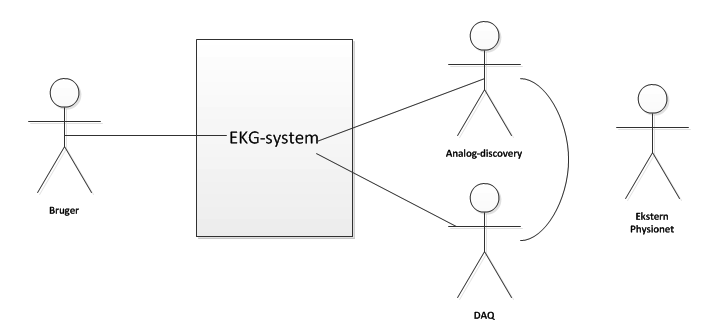
\includegraphics[width=1\textwidth]{Figurer/Snip20150409_30}
	\caption{Aktør-kontekstdiagram}
	\label{fig:aktoerbeskrivelse}
\end{figure}

Data hentes ned fra den ekstern aktør, physionet, og via Analog-discovery omdannes csv-filens data til et analogt signal, der sendes til EKG-systemet. Ud fra disse data danner EGK-systemet en graf. Programmet detekterer markørudsving i EKG-grafen, som derefter valideres og analyseres af brugeren.

\subsection{Aktørbeskrivelse}

\begin{table}[H]
\begin{tabularx}{\textwidth}{l l X}
     Aktørnavn  & Type      & Beskrivelse \\ \midrule
     Bruger   & Primær    & Brugeren er den aktør, der ønsker at foretage målingerne, som omfatter EKG samt diagnosticering af artieflimmer. Brugeren er en person, der har kendskab til EKG-systemet. Fx sundhedsfaglig personale \\ 						  									  \addlinespace[2mm]
     Analog-discovery & Sekundær  & Analog-discovery omdanner data fra den eksterne aktør, physionet, til et analog signal \\ 
     	\addlinespace[2mm]
     DAQ & Sekundær  & DAQ'en omdanner det analoge signal fra analog-discovery til et digitalt signal, som EKG-systemet kan generere en graf ud fra  \\ 
     	\addlinespace[2mm]
     Physionet & Ekstern 	& Physionet er en database, hvor der ligger mange forskellige EKG-signaler. Det er ud fra disse EKG-signaler, virtuelle patienter skabes.\\	                                                                                                                                                                           
   
     \bottomrule                                                                                                                   
    \end{tabularx}
    \caption {Aktørbeskrivelse}
    \label{tab:aktoerbeskrivelse}
	
\end{table}

\subsection{Use case-diagram}

\begin{figure}[htb]
	\centering
	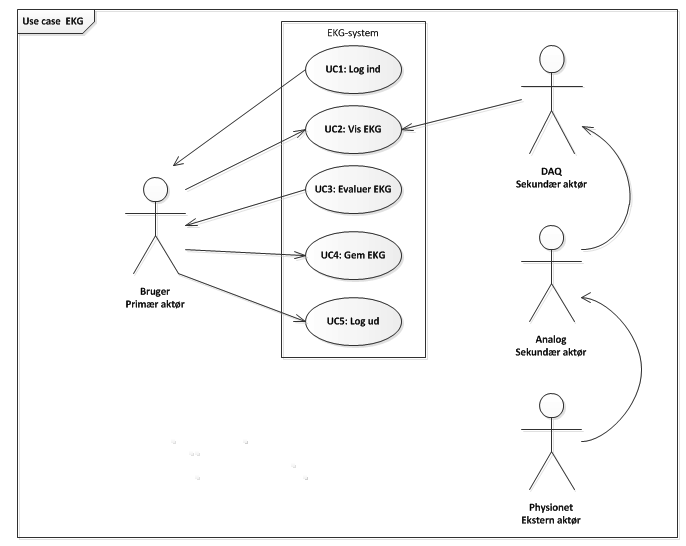
\includegraphics[width=1\textwidth]{Figurer/Snip20150327_24}
	\caption{Use case-diagram}
	\label{fig:Use Cases}
\end{figure}

Brugeren, den primære aktør bliver bedt om sit log ind, inden EKG-vinduet vises. Brugeren vælger indstillinger og trykker på "start"-knappen. EKG-dataerne fra den eksterne aktør, Physionet, behandles i Analog samt i DAQ'en, de sekundære aktør, hvor efter data vises som en EKG-graf i EKG-vinduet. Brugeren kan ud fra denne graf evaluere EKG-signalet i forhold til at diagnosticere atrieflimmer. Brugeren gemmer EKG-målingen i databasen og logger ud. 

\subsection{Use Cases}

\begin{longtabu} to \linewidth{@{}l r X[j]@{}} %UC1%
    {\large \textbf{Use Case 1}} && \\
    \toprule
    Navn &&    Log ind\\
    Use case ID &&    1\\
    Samtidige forløb &&    1\\
    Primær aktør &&    Brugeren\\
    Initialisere &&    Brugeren ønsker at logge ind\\
    Forudsætninger &&  At der er logget ud efter en tidligere måling\\
    Resultat &&    Brugeren bliver logget på og kan foretage en måling                     \\ \midrule
    Hovedforløb &    1. &    Brugeren indtaster username samt password\\[-1ex]   						 	
                &    2. &    Brugeren trykker på "Login-knappen". Login-vinduet lukkes ned mens CPR-vinduet åbnes\newline
                	[2.a \textit{Username eller password er forkert}]\\[-1ex]
                &    \\ \midrule
                
    Undtagelser &    2a. & Besked vises på skærmen med tekst, der informerer om, at username eller password er forkert. Der forsættes i UC1 ved punkt 1     \\ \bottomrule
\caption{Fully dressed Use Case 1.}
\label{UC1}
\end{longtabu}

\begin{longtabu} to \linewidth{@{}l r X[j]@{}} %UC2%
    {\large \textbf{Use Case 2}} && \\
    \toprule
    Navn &&    Vis EKG\\
    Use case ID &&    2\\
    Samtidige forløb &&    1\\
    Primær aktør &&    Brugeren\\
    Sekundær aktør &&	Analog\\
    Sekunær aktør &&	DAQ\\
    Ekstern aktør &&	Physionet\\
    Initialisere &&    Brugeren ønsker at foretage en EKG-måling\\
    Forudsætninger &&    Brugeren er logget ind og EKG-vinduet er vist samt Analog og DAQ'en er koblet til og data er hentet ned\\
    Resultat &&    EKG-graf bliver vist           \\ \midrule
    Hovedforløb &    1. &    Brugeren indtaster virtuel patients CPR-nummer\newline
    						 [1.a \textit{CPR-nummeret findes ikke}]\\[-1ex]
    			&    2. &    Brugeren vælger indstillinger\newline
    						 [2.a \textit{Brugeren er tilfreds med default-indstillingerne}]\\[-1ex]	
                &    3. &    Målingen startes ved at trykke på "Start"\\[-1ex]
                &    4. &    EKG-data illustreres på en graf\\ \midrule
                
    Undtagelser &    1a. &    CPR-nummeret findes ikke. Besked vises på 								skærmen med tekst, der informerer om, at CPR-						nummeret ikke er gyldigt. UC2 startes forfra 						med nyt CPR-nummer\\
    			&    2a. &    Der blev ikke ændret i default-indstillingerne. 				Der fortsættes ved punkt 2 i hovedforløbet med 				default indstillingerne
     \\ \bottomrule
\caption{Fully dressed Use Case 2.}
\label{UC2}
\end{longtabu}

\begin{longtabu} to \linewidth{@{}l r X[j]@{}} %UC3%
    {\large \textbf{Use Case 3}} && \\
    \toprule
    Navn &&    Evaluer EKG\\
    Use case ID &&    3\\
    Samtidige forløb &&    1\\
    Primær aktør &&    Brugeren\\
    Initialisere &&    Use Case 2 er gennemført   \\
    Resultat &&   Brugeren kan ud fra EKG-graf diagnosticere sygdommen atrieflimmer  \\ \midrule
    Hovedforløb &    1. &    Brugeren validere programmets analyse af EKG-signalet \\[-1ex]	
                &    2. &    Brugeren stiller diagnosen atrieflimmer\newline
                			 [2.a \textit{Atriefrekvensen er ikke i intervallet 220-300 pr. minut}]\\ \midrule
                
    Undtagelser &    2a. &    Det er ikke muligt at diagnosticere atrieflimmer ud fra grafen. Use case 3 afsluttes og Use case 2 gentages med evt. nye tidsindstillinger \\ \bottomrule
\caption{Fully dressed Use Case 3.}
\label{UC3}
\end{longtabu}

\begin{longtabu} to \linewidth{@{}l r X[j]@{}} %UC4%
    {\large \textbf{Use Case 4}} && \\
    \toprule
    Navn &&    Gem EKG\\
    Use case ID &&    4\\
    Samtidige forløb &&    1\\
    Primær aktør &&    Brugeren\\
    Initialisere &&    Brugeren ønsker at gemme EKG i databasen\\
    Forudsætninger &&  Use case 3 er gennemført\\
    Resultat &&    EKG er gemt i databasen                    \\ \midrule
    Hovedforløb &    1. &    Brugeren trykker på "Gem-knappen". En messagebox kommer frem med besked om at data er gemt\\[-1ex]   						 	
                &    2. &	Brugeren trykker på "Ok" knappen for at lukke messageboxen og EKG-vinduet vises igen
                	\\ \midrule
                
    Undtagelser &       \\ \bottomrule
\caption{Fully dressed Use Case 4.}
\label{UC4}
\end{longtabu}

\begin{longtabu} to \linewidth{@{}l r X[j]@{}} %UC5%
    {\large \textbf{Use Case 5}} && \\
    \toprule
    Navn &&    Log ud\\
    Use case ID &&    5\\
    Samtidige forløb &&    1\\
    Primær aktør &&    Brugeren\\
    Initialisere &&    Brugeren ønsker at logge ud\\
    Forudsætninger &&  Der skal være logget ind\\
    Resultat &&    Brugeren bliver logget ud, og EKG-vinduet lukkes og login-vinduet fremkommer                     \\ \midrule
    Hovedforløb &    1. &    Brugeren trykker på "log ud-knappen" og EKG-vinduet lukkes, mens login-vinduet fremkommer 
    \\ \midrule
    Undtagelser & &
         \\ \bottomrule
\caption{Fully dressed Use Case 5.}
\label{UC5}
\end{longtabu}

\section{Ikke-funktionelle krav}
De ikke-funktionelle krav er udarbejdet ved brug af (F)URPS+. De er alle prioriteret ved MoSCoW metoden - Must (skal være med), Should (bør være med, hvis muligt), Could (kunne have med, hvis det ikke influerer på andet), Won't/Would (ikke med nu, men med i fremtidige opdateringer). 

\subsection{(F)URPS+}
MoSCoW er angivet i parentes med hhv. M, S, C eller W.

\textbf{Usability}
\begin{itemize}
	\item (M) Brugeren skal kunne starte en default-måling maksimalt 20 sek. efter opstart af programmet
	\item (M) Brugeren skal have mulighed for at ændre tidsintervallet før målingerne foretages
	\item (M) Login-vinduet skal indholde en "login"-knap til at logge på og få vist EKG-vinduet
	\item (M) EKG-vinduet skal indeholde en "start"-knap til at igangsætte målingerne
	\item (M) EKG-vinduet  skal indeholde en "stop"-knap til at afslutte målingerne før den valgte tid
	\item (M) EKG-vinduet skal indeholde en "log ud"-knap
	\item (M) EKG-vinduet  skal indeholde en "gem"-knap
	\item (M) Information-vinduet skal indeholde en "gem"-knap
	\item (M) Målingen stopper automatisk efter det valgte tidsinterval
\end{itemize}

\textbf{Reliability}
\begin{itemize}
	\item (M) Systemet skal have en effektiv MTBF (Mean Time Between Failure) på 20 minutter og en MTTR (Mean Time To Restore) på 1 minut.
				\begin{align}
					Availability = \frac{MTBF}{MTBF+MTTR} = \frac{20}{20+1} = 0,952 = 95,2 \%
				\end{align}

\end{itemize}

\textbf{Performance}
\begin{itemize}
	\item (M) Der skal vises en EKG-graf i EKG-vinduet, hvor spænding vises op af y-aksen (-1V til 1V) og tiden på x-aksen
	\item (M) Grafen skal være scrollbar på x-aksen, så brugeren selv ved brug af musen kan vælge det udsnit af grafen, der skal vises mere detaljeret
	\item (M) Skal tage en sample over et brugerbestemt interval, hvor frekvensen  er tilpasset målingerne, således at grafen er analyserbar
\end{itemize}

\textbf{Supportability}
\begin{itemize}
	\item (M) Softwaren er opbygget af trelagsmodellen
\end{itemize}















